\documentclass[12pt]{report}
\usepackage[a4paper]{geometry}
\usepackage{fancyhdr}
\usepackage{lastpage}
\usepackage{graphicx, wrapfig, subcaption, setspace, booktabs}
\usepackage[T1]{fontenc}
\usepackage[font=small, labelfont=bf]{caption}
\usepackage{fourier}
\usepackage[protrusion=true, expansion=true]{microtype}
\usepackage[english]{babel}
\usepackage{sectsty}
\usepackage{url, lipsum}
\usepackage{enumitem}

\graphicspath{ {img/} }
\newcommand{\HRule}[1]{\rule{\linewidth}{#1}}
\renewcommand{\headrulewidth}{0pt}
\linespread{2}

%-------------------------------------------------------------------------------
% HEADER & FOOTER
%-------------------------------------------------------------------------------
% \pagestyle{fancy}
% \fancyhf{}
% \fancyhead[L]{Student ID: 20550430}
% \fancyhead[R]{University of Waterloo}
% \fancyfoot[C]{\thepage} % / \pageref{LastPage}

%-------------------------------------------------------------------------------
% TITLE PAGE
%-------------------------------------------------------------------------------

\begin{document}
\begin{titlepage}
   \begin{center}
    	\normalsize \textbf{\uppercase{University of Waterloo}} \\
		Faculty of Mathematics \\
	\end{center}	
		\vspace*{\stretch{0.1}}
	\begin{center}
		\HRule{0.5pt}
   		\LARGE \textbf{\uppercase{Scaling Messaging Queues}}
   		\HRule{0.5pt}
	\end{center}
	\vspace*{\stretch{0.1}}
	\begin{center}
	   		\normalsize {ARB Labs\\ Niagara Falls, Ontario}	
	 
	\end{center}
	\vspace*{\stretch{0.1}}
	\begin{center}
	   		\normalsize {Prepared by\\
				Nicholas Westbury\\
				3A Computer Science\\
				ID 20550430\\
	   		 	\today
	   		 }
	\end{center}
\end{titlepage}

\newpage\noindent\thispagestyle{empty}
\LARGE\textbf{\uppercase{MEMORANDUM}} \normalsize
\vspace*{-10px}
\begin{singlespacing}\noindent
\vspace*{-10px}
To: Vlad Cazan\\
\vspace*{-10px}
From: Nicholas\\
\vspace*{-10px}
Date: \today\\
\vspace*{-10px}
Re: Work Report: Scaling Systems\\
\end{singlespacing}
\HRule{1.5pt}\\
I have prepared the enclosed report, "Scaling Messaging Queues" for my 3A work report. This is the second of four work reports that the Co-operative Education Program required as part of Co-op degree requirements. As you are aware, one of my primary duties as a Python Developer for Winter 2016 was to improve ARB Lab's messaging system. This report is an exploration of our implementation and the thought behind some of the design decisions.\\ \\ \noindent
As part of this process, the Faculty of Mathematics requests that you evaluate this report for command of topic and technical content/analysis. Your evaluation will be submitted to the Math Undergrad Office for evaluation. The combined marks determine whether the report will receive credit. \\ \\
Thank you for your help in preparing this report,\\ \\ \noindent

\includegraphics[scale=0.55]{signature}

\newpage\thispagestyle{fancy}\sectionfont{\scshape}
\section*{Table of Contents}
\normalsize
\begin{enumerate}[label={},leftmargin=*,labelsep=2ex]
    \item 1.0 Introduction \dotfill 1
    \item 2.0 Analysis \dotfill 2
    \item 2.1 Introduction to Messaging Queues \dotfill 2
    \item 2.2 Comparison of Messaging Queues \dotfill 4
      \begin{enumerate}[label*={},leftmargin=*,labelsep=2ex]
        \item 2.2.0 Fault Tolerance and Queue Persistence \dotfill 4
        \item 2.2.1 Configuration Complexity \dotfill 4
        \item 2.2.2 Throughput vs Median Message Speed \dotfill 5
      \end{enumerate}
    \item 2.3 Information Flow \dotfill 7
    \item 2.4 Module Abstraction \dotfill 9
    \item 2.5 Message Stability \& Security \dotfill 11
    \begin{enumerate}[label*={},leftmargin=*,labelsep=2ex]
        \item 2.5.0 Message Consistency \dotfill 11
        \item 2.5.1 Message Security \dotfill 12
      \end{enumerate}
    \item 3.0 Conclusion \dotfill 13
    \item 4.0 References \dotfill 14
\end{enumerate}
\fancyfoot[C]{ii}

\newpage\thispagestyle{fancy}\sectionfont{\scshape}
\section*{List of Figures}
\normalsize\cfoot{3aa}
\begin{enumerate}[label=\arabic*,leftmargin=*,labelsep=2ex,ref=\arabic*]
    \item Messaging Queues Diagram \dotfill 2
    \item Comparison of Messaging Queue Platforms \dotfill 6
    \item Data Flow Diagram \dotfill 8
    \item Authentication Flow Diagram \dotfill 12
\end{enumerate}

\fancyfoot[C]{iii}

\newpage\thispagestyle{fancy}\sectionfont{\scshape}
\section*{Executive Summary}
What do Facebook, Microsoft, Google and most technology companies have in common? Each handles huge amounts of internet traffic, with as much as thousands of requests per second (1). Systems are specially designed from the ground up to handle the volume and speed of these requests. Our system at ARB Labs relies on a messaging system to handle the communication across a network of modules. \\ \\ \noindent
This report will analyze the design decisions of ARB Labs' newly revamped messaging and classification system, considering both the advantages and drawbacks of key decisions. In particular, the ease of development, speed, and security will be discussed. Leaving a clear understanding of the functionality and justifications for implementation decisions.

\fancyfoot[C]{iv}

%-------------------------------------------------------------------------------
% BODY
%-------------------------------------------------------------------------------

\newpage\thispagestyle{fancy}\sectionfont{\scshape}

% Reset the page counter
\setcounter{page}{1}
\fancyfoot[C]{\thepage}

\section*{1.0 Introduction}
\addcontentsline{toc}{section}{Introduction}
\par\indent
ARB Labs was founded as a gesture-recognition company but soon expanded to image recognition when they found a shortcoming in the casino market. Historically, casino pit bosses would manually track the amount of each player's bet. This data collection method is both time consuming and error-prone. As a solution, ARB Labs developed an innovative bet recognition system that captures images of the chips in the bet area of the tables,  classifying the colour and value of each of the casino chips using a machine learning algorithm. The system is composed of a small computer cluster installed directly onto existing casino tables with a remote classification server.\\ \\ \noindent
From a technical standpoint, it is critical of that the system is reliable, fast, and secure. To accomplish these goals, the various computers need to be able to communicate amongst each other effectively. Messaging queues is one popular way to communicate across processes. This report will concentrate primarily on exploring the decisions made to improve the system's backend, with particular emphasis on messaging between the system components. \\ \par\noindent

\newpage\thispagestyle{fancy}\sectionfont{\scshape}
\section*{2.1 Introduction to Messaging Queues}
\addcontentsline{toc}{section}{Introduction}
\par\indent
Messaging queues are one of the most popular methods to communicate between processes or computers. A basic messaging queue is composed of two major components, a producer (also called a publisher) and a consumer (also known as a subscriber). As the name implies, the role of a producer is to send a message to a consumer queue. The consumer then pops messages from its queue and reads them in the order they were sent from the producer (generally speaking).
\\ \\
\begin{figure}[h]
\centering
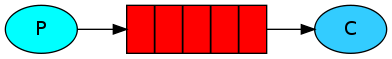
\includegraphics{simple_queue}
\caption{A producer $P$ produces to a queue which is read from consumer $C$.}
\end{figure}
\\ \\
Many implementation details are left to individual messaging queue software and configurations. Some important implementation-specific details include:
\begin{itemize}
  \item The delivery method used to pass messages from a producer to consumer. For example Hypertext Transfer Protocol (HTTP), Transmission Control Protocol (TCP), and Secure Shell (SSH) are all possible transportation protocols.
  \item The queue durability after a message is received can either be persistent storing the messages or temporary for real-time queues.
  \item When a producer sends a message can either be sent directly to a single queue or to multiple queues. The messaging queue can have an "exchange" and a "routing key" to determine which queue(s) to deliver the message to. 
  \item Information is generally passed unilaterally from a producer to a consumer. However, a process can be both a producer and a consumer if using the request/reply messaging pattern, allowing for indication when a message was successfully received by a consumer.
  \item Messages can be sent individually or in batches.
\end{itemize}
 
\newpage\thispagestyle{fancy}\sectionfont{\scshape}
\section*{2.2 A Comparison of Messaging Queues}
\addcontentsline{toc}{section}{Introduction}
\par\indent
Our system considered three different software project implementing queues: Redis, Kafka, and RabbitMQ. Each of these products work differently and offer unique advantages and drawbacks.

\subsection*{2.2.0 Fault Tolerance and Queue Persistence}

One important consideration for our system is the fault tolerance. We will be deploying our system to remote locations and therefore have the ability to easily perform on-site maintenance. There is a requirement for the queues to recover from their queues if there are still messages in transition when the system fails and is rebooted. In the Redis messaging queue all messages are stored in-memory by default. This means that if the consumer computer loses power then all messages would be lost, leaving the system in an unstable state. On the other hand, if the queue is persistent then the messages can recover on reboot. Queue persistence is possible in both Kafka and RabbitMQ.

\subsection*{2.2.1 Configuration Complexity}

On Kafka, queue configuration is primarily done on each of the brokers where the messages are sent. On the other hand, Redis allows for most of the configuration to be done on per-queue basis and RabbitMQ on a per-exchange basis. From a practical standpoint, it is more convenient to set a smaller number of settings for each of the queues than to configure the hundreds of options available on Kafka on each broker (2).

\subsection*{2.2.2 Throughput vs Median Message Speed}

Counterintuitively, the throughput and message received speed are not the same. After benchmarking Kafka, it was apparent that although it has the highest throughput and the lowest \textit{average} message received time it did not necessarily have the lowest median message speed for our binary image data. By default, Kafka sends multiple messages in a single compressed message, thereby increasing throughput when there is a constant stream of messages. However, when the messages are sent more slowly, the median time to receive the message is higher because the Kafka broker unsuccessfully waits to combine the messages. In our particular case, data traffic is sent in short bursts of multiple messages. Although RabbitMQ features a lower throughput, its lower median message time made it a better fit for this task.\\

\newpage

In summary, each messaging queue platform has its own advantages and drawbacks. Redis is the easiest message queue platform to develop in but it lacks the speed and full queue persistence. Kafka is flexible and extendable but can be difficult to configure. RabbitMQ is a middle ground between these platforms. The following table summarizes the significant differences between the systems:

\begin{center}
\begin{tabular}{ |c|c|c|c| }
 \hline
 \textbf{Name} & \textbf{Redis} & \textbf{Kafka} & \textbf{RabbitMQ} \\ \hline
 Queues Persistence & In-memory & Persistent & Persistent\\ \hline
 Fault Tolerance & Low & High & High\\ \hline
 Replication & By Queue & By Broker  & By Queue \\ \hline
 Design Complexity & Low & High & Low \\ \hline
 Throughput & Medium & High (network limit) & Medium \\ \hline
 Message Speed & High & Medium (batched) & High \\ \hline 
\end{tabular}
\end{center}
\begin{figure}[h]
\caption{A comparison between popular messaging queues platforms}
\end{figure}

\newpage\thispagestyle{fancy}\sectionfont{\scshape}
\section*{2.3 Information Flow}
\par

The way the system communicates with each of its components is one of particular interest. There are two broad divisions to our table system: the camera capturing component and the displaying component. The camera capturing component is itself composed of a camera cluster, four small computers that control these cameras, and a "handcount" unit: a proximity sensor activated at the start of each new hand when a card is placed on top of it. The display component is composed of two screens and a magnetic reader, used for logging in players and dealers when they swipe their identification cards. Each table also communicates with a central database which handles the image classification, login handling, and log collecting.

To understand the system structure, it is crucial to understand the information being transmitted between the system's components. There are four steps: login, hand start signal, evaluation, and displaying the evaluation. Each step in this process communicates with at least one other consumer or producer and in a strict chronological order.

\begin{enumerate}
  \item First the player and dealer are logged into the system using a magnetic reader. This produces a message to the screen which then produces a login message to the database. If the database successfully issues the login, the player's credentials are displayed on the screen.
  
  \item When a hand is going to start, the handcount unit is activated producing a message to the camera controller consumer. The camera controller then produces to a message to all cameras triggering them to capture images.
  
  \item Each of the four cameras then send their images to the server for evaluation.
  
  \item The server finally sends the chip amounts for each of the images to the two screens.

\end{enumerate}

This data flow is summarized in the diagram below:
\begin{figure}[h]
\centering
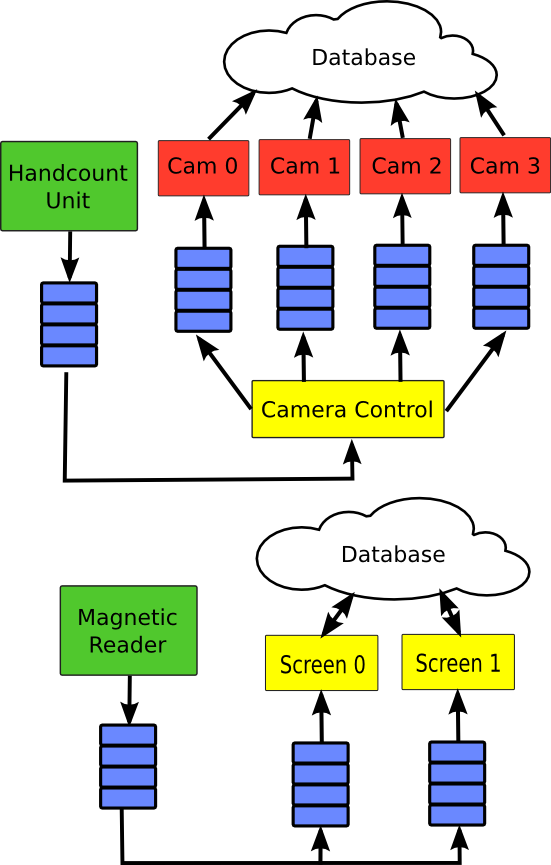
\includegraphics[scale=0.50]{system_diagram}
\caption{A summary of the system where the consumers are in red, the producers are in green, and a combination of both are in yellow. Consumer queues are in blue.}
\end{figure}

\newpage\thispagestyle{fancy}\sectionfont{\scshape}
\section*{2.4 Module Abstraction}

\subsection*{2.4.0 Modularity}
One of the requirements of our system is the ability to easily swap out components tailored to particular clients' needs. For instance, a particular casino can request to have a different database system, such as MySQL (Structured Query Language), instead of our default MongoDB. To accommodate this type of change, we chose to use the object-oriented paradigm with fully virtual classes for most of our classes (3). This model is similar to Java's interface where only function signatures are declared and a separate class implements these methods. \\ \\
Since our code base is written almost exclusively in Python, we utilized the "abc" module to allow for virtual methods to be declared. This allows the multiple database connectors to inherit from a database connector interface that has high-level functions such "insert\_into\_database" or "fetch\_from\_database". With this code organization, implementing different versions is simply a matter of implementing those methods.

\subsection*{2.4.1 Modules as Message Relays}
Another property of the system is that each of the many physical components are sufficiently abstracted, such that they can be treated essentially as a consumer and/or producer, without the need to understand how the message is sent. The only knowledge that may change between modules is the message format. Once the message format is known, the consumer doesn't need to concern itself with how it was sent or implemented internally. The message-only communication creates strong distinction between modules, and therefore lowers the coupling of the modules, making it easier to maintain and read each module's code (Warren 4).

\newpage\thispagestyle{fancy}\sectionfont{\scshape}
\section*{2.5 Message Stability \& Security}

\subsection*{2.5.0 Message Consistency}
Usually having synchronized messages is not an issue for most of our components, since they are stateless and act completely independently. For example, cameras simply capture image when they receive a capture message. However, for authentication a more sophisticated message handling is needed since there are two components, in this case, the screen and the database. These two components need to have a synchronized state. Having atomic transaction, where either the entire login or logout operation happens, or nothing at all is required to maintain consistency (Niemeyer 5). This is crucial to maintain synchronization. \\ \\
With our distributed model, implementing a truly atomic authentication transaction is surprisingly complex. To handle the vast majority of cases, the screen should update its status only after receiving a response from the database with whether the authentication was issued or not. With a response from the database, the screen is known to have the login state as the database. In addition to responding to each authentication request a timeout for each message is implemented. For example, the screen updates only on a positive database response if a response is received within the timeout period. This pattern, called a request-reply pattern, is common in web development but less common in messaging queues.
\begin{figure}[h]
\centering
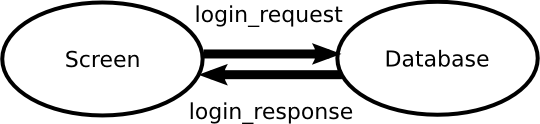
\includegraphics[scale=0.55]{communication}
\caption{The request/reply pattern}
\end{figure}
\noindent
Although this simple model is far better than no response at all, it is not truly transactional, since there are rare cases where the system could enter an inconsistent state. For example, if the screen was to fail after sending a message but before a database response then the screen and database would differ in state. The traditional solutions are either to maintain high uptime, to workaround the issue entirely, or have a central broker to issue transactions (Kaye 6). Given the additional complexity required to have a central broker and the extremely low probability of failure, a fully-transactional system makes only sense in contexts where correctness is mission critical.

\subsection*{2.5.1 Message Security}
Message security is another important consideration. In particular, a system should ensure that there cannot be a man-in-middle attack where a malicious computer can intercept and potentially modify the message while in transit. RabbitMQ makes it easy to implement Transport Layer Security (TLS) with RSA encryption, the same encryption that is used by websites to encrypt HTTP requests. With this encryption, it is impractical to read any intercepted message because it would take an estimated 6.4 quadrillion years of computing time to crack the 2048 bit RSA (7).

\newpage\thispagestyle{fancy}\sectionfont{\scshape}
\section*{3.0 Conclusion}
\addcontentsline{toc}{section}{Conclusion}
\par\indent
Of the possible methods to relay information from physical components, messaging queues have proven to be a flexible and effective solution. It is fast, secure, and has good object-oriented properties. The drawbacks when it comes to messaging speed and message stability can be worked around. The ability to handle thousands of requests per second across multiple devices can be done with ease.

 \noindent

%-------------------------------------------------------------------------------
% REFERENCES
%-------------------------------------------------------------------------------
\newpage
\section*{4.0 References}
\addcontentsline{toc}{section}{References}

\begin{enumerate}
\item "Google Search Statistics." Google Search Statistics - Internet Live Stats. N.p., n.d. Web. 15 Apr. 2017.
\item "Documentation." Apache Kafka. N.p., n.d. Web. 15 Apr. 2017.
\item "RabbitMQ Documentation." RabbitMQ. N.p., n.d. Web. 15 Apr. 2017.
\item "abc - Abstract Base Classes." abc - Abstract Base Classes - Python 2.7.13 documentation. N.p., n.d. Web. 15 Apr. 2017.
\item Matthew Warren. "High Cohesion, Loose Coupling." The Bojan's Blog. N.p., 8 Apr. 2015. Web. 15 Apr. 2017.
\item Niemeyer, Patrick. Learning java. N.p. O'Reilly Media, 2017. Print.
\item Kaye, Doug. Loosely coupled: the missing pieces of Web services. Marin County, CA: RDS Press, 2003. Print.
\item "The Math Behind Estimations to Break a 2048-bit Certificate." Just How Strong is 2048-bit SSL Certificate Encryption? N.p., n.d. Web. 15 Apr. 2017.
\end{enumerate}

\end{document}